\documentclass[preview]{standalone}

\usepackage{amsmath}
\usepackage{amssymb}
\usepackage{tikz}
\usepackage{wrapfig}
\usepackage{bettelini}
\usepackage{stellar}
\usepackage{definitions}

% =======
\usetikzlibrary{ % tikz packages
    automata,positioning,
    arrows.meta,bending
}
\tikzset{every state/.style={
    inner sep=2pt,
    minimum size=4pt
}}
\tikzset{>=stealth}  %latex, to, stealth
% Empty string symbol.
\newcommand{\emptyString}{\lambda}
% =======

\begin{document}

\id{theoryofcomputation-regexpr-vs-dfa}
\genpage

\section{Equivalence of regular expressions and regular languages}

\begin{snippettheorem}{reg-expr-desc-reg-lang}{Regular expressions describe regular languages}
    Any regular expression descrive a regular language.
\end{snippettheorem}

\begin{snippetproof}{reg-expr-desc-reg-lang-proof}{Regular expressions describe regular languages}
    Let \(R\) be a regular expression over \(\Sigma\).

    \begin{wrapfigure}{r}{2.5cm}
        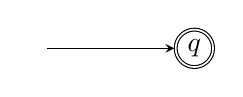
\begin{tikzpicture}[node distance=2cm,on grid,auto]
            \node[state, accepting] (q) {\(q\)};
            \node (inv) [left=of q] {};
        
            \path[->]
                (inv)
                    edge node {} (q);
        \end{tikzpicture}
    \end{wrapfigure}

    Assume that \(R=\emptyString\). Then \(R\) describes \(\{\emptyString\}\).
    This language is regular and we can prove it by constructing an NFA \(N=(Q, \Sigma, \delta, q, F)\)
    such that \(L(N)=\{\emptyString\}\).
    \(q\) is the start state, \(Q=\{q\}\), \(F=\{q\}\) and \(\delta(r,a)=\emptyset\)
    where \(a\in\Sigma_\emptyString\).
    \wrapfill

    \begin{wrapfigure}{r}{2.5cm}
        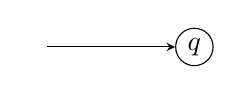
\begin{tikzpicture}[node distance=2cm,on grid,auto]
            \node[state] (q) {\(q\)};
            \node (inv) [left=of q] {};
        
            \path[->]
                (inv)
                    edge node {} (q);
        \end{tikzpicture}
    \end{wrapfigure}

    Assume that \(R=\emptyset\). Then \(R\) describes \(\emptyset\).
    This language is regular and we can prove it by constructing an NFA \(N=(Q, \Sigma, \delta, q, F)\)
    such that \(L(N)=\emptyset\).
    \(q\) is the start state, \(Q=\{q\}\), \(F=\emptyset\) and \(\delta(r,a)=\emptyset\) where \(a\in\Sigma_\emptyString\).
    \wrapfill

    \begin{wrapfigure}{r}{2.5cm}
        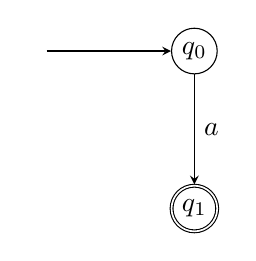
\begin{tikzpicture}[node distance=2cm,on grid,auto]
            \node (inv) {};
            \node[state] (q0) [right=of inv] {\(q_0\)};
            \node[state, accepting] (q1) [below=of q0] {\(q_1\)};
        
            \path[->]
                (inv)
                    edge node {} (q0)
                (q0)
                    edge node {\(a\)} (q1);
        \end{tikzpicture}
    \end{wrapfigure}

    Assume that \(R=a\) where \(a\in\Sigma\). Then \(R\) describes \(\{a\}\).
    This language is regular and we can prove it by constructing an NFA \(N=(Q, \Sigma, \delta, q, F)\)
    such that \(L(N)=\{a\}\).
    \(q_0\) is the start state, \(Q=\{q_0, q_1\}\), \(F=\{q_1\}\) and
    \[
        \delta(r,b \in) =
        \begin{cases}
            \{q_1\} & b=a \land r=q_0\\
            \emptyset & \text{otherwise}
        \end{cases}
    \]
    where \(b\in\Sigma_\emptyString\).
    \wrapfill

    Assume that \(R=R_1 \union R_2\) where \(R_1\) and \(R_2\) are regular expressions.
    Let \(L_1\) and \(L_2\) be the languages described by \(R_1\) and \(R_2\) respectively.
    Assuming that \(L_1\) and \(L_2\) are regular, \(R\) then describes \(L_1 \union L_2\) which by theorem is regular.

    Assume that \(R=R_1 \intersection R_2\) where \(R_1\) and \(R_2\) are regular expressions.
    Let \(L_1\) and \(L_2\) be the languages described by \(R_1\) and \(R_2\) respectively.
    Assuming that \(L_1\) and \(L_2\) are regular, \(R\) then describes \(L_1 \intersection L_2\) which by theorem is regular.

    Assume that \(R=R_1 R_2\) where \(R_1\) and \(R_2\) are regular expressions.
    Let \(L_1\) and \(L_2\) be the languages described by \(R_1\) and \(R_2\) respectively.
    Assuming that \(L_1\) and \(L_2\) are regular, \(R\) then describes \(L_1 L_2\) which by theorem is regular.

    Assume that \(R={(R_1)}^*\) where \(R_1\) is a regular expression. Let \(L_1\) be the language be described
    by \(R_1\). Assuming that \(L_1\) is regular, then \(R\) describes \({(L_1)}^*\) which by theorem is regular.

    Assume that \(R=\bar{R_1}\) where \(R_1\) is a regular expression. Let \(L_1\) be the language be described
    by \(R_1\). Assuming that \(L_1\) is regular, then \(R\) describes \(\bar{L_1}\) which by theorem is regular.

    This proves that every regular expression describes a regular language since every
    regular expression can be broken down to regular languages.
\end{snippetproof}

\subsection{A DFA can be converted into a regular expression}

\subsubsection{Solving recurrence relations}

\begin{snippetlemma}{recurrence-relations-language}{Recurrence relation}
    Let \(\Sigma\) be an alphabet and let \(B\), \(C\) and \(L\) be languages in \(\Sigma^*\) where \(\emptyString \notin B\)
    \[
        L=BL\union C \implies L=B^*C
    \]
\end{snippetlemma}

\begin{snippetlemma}{recurrence-relations-language-proof}{Recurrence relation}
    In order to prove this we first show that \(B^*C \subseteq L\) by induction.
    Let \(w \in B^*C\), then \(w\) is \(k\geq 0\) strings in \(B\) followed a string in \(C\).
    When \(k=0\), \(w \in C\) which implies \(w \in BL\union C\) which implies \(w \in L\).
    When \(k > 0\) we can write \(w\) as \(xyz\) where \(x\) is a string in \(B\),
    \(y\) is the concatenation of \(k-1\) strings in \(B\) and \(c \in C\).
    Let \(q=yz\). Since \(q\) is a concatenation of \(k-1\) strings of \(B\) followed by a string in \(C\),
    \(q \in L\). Hence, \(w=xq\) where \(x\in B\) and \(q\in L\). This shows that \(w \in BL\).
    Hence, \(w \in BL\union C\). Since \(BL \union C = L\), \(w \in L\). This proves that
    \(B^*C\subseteq L\). \\
    Now we show that \(L \subseteq B^*C\) by induction to conclude the proof.
    Let \(w\in L\). When \(|w|=0\), \(w=\emptyString\). Since \(\emptyString \notin B\),
    \(w \notin BL\). This means that \(w\in C\). Since \(C \subseteq B^*C\) the string \(w\)
    is also in \(B^*C\). When \(|w| > 0\), if \(w \in C\) then \(w \in B^*C\),
    If \(w \notin C\), \(w \in BL\) since \(w \in L\) and \(L=BL\union C\).
    Hence, \(w=bl\) where \(b\in B\) and \(l\in L\).
    Since \(\emptyString \notin B\), \(|b|>0\). This means that \(|l|<|b|\)
    since \(|l|+|b|=|w|\). By induction, \(l\) is a string in \(B^*C\).
    Hence, \(w = bl\) where \(b\in B\) and \(l\in B^*C\). This shows that \(w \in B(B^*C)\).
    Since \(B(B^*C) \subseteq B^*C\) it follows that \(w \in B^*C\).
\end{snippetlemma}

\subsubsection{The conversion}

\begin{snippettheorem}{dfa-to-regular-expr}{DFA to regular expression}
    Every DFA can be converted into a regular expression.
\end{snippettheorem}

\begin{snippetproof}{dfa-to-regular-expr-proof}{DFA to regular expression}
    Let \(M=(Q, \Sigma, \delta, q, F)\) be a DFA. We will prove that there exists a regular
    expression describing \(L(M)\).
    
    We define \(L_r\) where \(r \in Q\) as the set of strings \(w \in \Sigma_\emptyString\)
    that would be accepted by \(M\) if \(r\) were its start state, meaning the language of \(M\)
    if \(r\) were its start state. Note that \(L(M)=L_q\).
    TODO
\end{snippetproof}

\subsection{Conclusion}

\begin{snippettheorem}{language-regular-is-regular-expr}{Regular expression and regular languages}
    A language \(L\) is regular iff there exists a regular expression that describes \(L\).
\end{snippettheorem}

\begin{snippetproof}{language-regular-is-regular-expr-proof}{Regular expression and regular languages}
    Since any DFA \(M\) can be converted into a regular expression that describes \(L(M)\)
    and every regular expression describes a regular language, we can conclude that a language \(L\)
    is regular iff there exists a regular expression that describes \(L\).
\end{snippetproof}

\end{document}